%Jennifer Pan, August 2011

\documentclass[10pt,letter]{article}
	% basic article document class
	% use percent signs to make comments to yourself -- they will not show up.

\usepackage{amsmath}
\usepackage{amssymb}
\usepackage{tikz}
	% packages that allow mathematical formatting

\usepackage{graphicx}
	% package that allows you to include graphics

\usepackage{setspace}
	% package that allows you to change spacing

\onehalfspacing
	% text become 1.5 spaced

\usepackage{fullpage}
	% package that specifies normal margins

\renewcommand{\vector}[1]{\boldsymbol{#1}}
\newcommand{\problem}[1]{\section*{Problem #1}}
\newcommand{\problempart}[1]{\paragraph{#1}}

\begin{document}
	% line of code telling latex that your document is beginning


\title{Problem Set 3}

\author{Nicholas Wu}

\date{Fall 2020}
	% Note: when you omit this command, the current dateis automatically included

\maketitle
	% tells latex to follow your header (e.g., title, author) commands.
\textbf{Note:} I use bold symbols to denote vectors and nonbolded symbols to denote scalars. I primarily use vector notation to shorthand some of the sums, since many of the sums are dot products.

\problem{1}

\problempart{(1)}
The optimal time length of schooling maximizes:
\[ \max_S \int_S^\infty e^{-(r + \nu)t}w(t)h(t) \]
\[ \max_S \int_S^\infty e^{-(r+ \nu - g)t}S^{\alpha} \]
\[ \max_S \frac{S^{\alpha}w(0)e^{-(r+ \nu-g)S}}{r-g} \]
\[ \frac{\alpha S^{\alpha - 1}}{S^\alpha} = r+ \nu-g\]
\[  S = \frac{\alpha}{r+ \nu-g} = 9\]
\problempart{(2)}
The present value of consumption is
\[ \int_S^\infty e^{-rt}c_t = \int_S^\infty w(0) e^{-(r-g)t}S^\alpha \]
\[  = \frac{w(0) e^{-(r-g)S}S^\alpha }{r-g}\]
\problempart{(3)}
We need
\[ \max  \int e^{-(\rho + \nu)t} \log c(t) \]
subject to
\[ \int e^{- rt}c(t) = \frac{w(0) e^{-(r-g)S}S^\alpha }{r-g} \]
we have
\[ e^{-(\rho + \nu)t} \frac{1}{c(t)} = \lambda e^{-rt}\]
\[ \frac{1}{\lambda }e^{-(\rho + \nu - r)t}  = c(t) \]
and we get the EE:
\[ \frac{\dot{c}(t)}{c(t)}= r - \rho - \nu  \]
which implies
\[ c(t) = c(0) e^{(r-\rho-\nu)t} \]
Plugging into budget constraint:
\[ \frac{c(0)}{\rho+\nu} = \frac{w(0) e^{-(r-g)S}S^\alpha }{r-g} \]
\[ c(0) = \frac{w(0)(\rho+\nu) e^{-(r-g)S}S^\alpha }{r-g} \]

\problempart{(4)}
Intuitively, since consumption is smoothed across time, individuals will go into debt before they reach their optimal level of schooling. Specifically, at time $T < S$, we have the present value of an individual's asset holding is given by
\[ -e^{rT}\int_0^T e^{-rt}c(t) \]
which is clearly negative. However, after the individual finishes schooling, the present value of asset holding is
\[ e^{rT}\left(\int_S^T e^{-rt} W_t dt - \int_0^T e^{-rt}c_t \right) \]
\[ = e^{rT}\left(w(0)S^{\alpha} \int_S^T e^{-(r-g)t} dt - c(0)\int_0^T  e^{-(\rho+\nu)t} \right) \]
\[ = e^{rT}\left(\frac{w(0)S^{\alpha}}{r-g} \left( e^{-(r-g)T} - e^{-(r-g)S}  \right)- \frac{w(0)(\rho+\nu) e^{-(r-g)S}S^\alpha }{r-g} \left(\frac{e^{-(\rho+\nu)T} - 1}{\rho+\nu}  \right) \right) \]
\[ = \frac{w(0)S^{\alpha}e^{rT}}{r-g}\left( \left( e^{-(r-g)T} - e^{-(r-g)S}  \right)-  e^{-(r-g)S} \left(e^{-(\rho+\nu)T} - 1  \right) \right) \]
\[ = \frac{w(0)S^{\alpha}e^{rT}}{r-g}\left(  e^{-(r-g)T} - e^{-(r-g)S} \left(e^{-(\rho+\nu)T} \right) \right) \]
\[ = \frac{w(0)S^{\alpha}e^{rT}e^{-(r-g)S}}{r-g}\left(   e^{-(r-g)(T-S)}- e^{-(\rho+\nu)T}  \right) \]
Since $r-g > \rho+\nu$, this will eventually turn positive at
\[ e^{-(r-g)(T-S) + (\rho + \nu)T} = 1 \]
\[ (r-g)(T-S) = (\rho + \nu)T \]
\[ (r-g - \rho - \nu)T = (r-g)S \]
\[ T = \frac{(r-g)S}{(r-g - \rho - \nu)} \]
so after that point, the individual paid of their student loans and will begin accummulating wealth.

\problempart{(5)}
If we take the $\log$ of the wage rate, we find that
\[ \log W(t) = \log w(0) + \alpha \log S + gt \]
which we can use to empirically measure the schooling effectivness parameter $\alpha$.
\problempart{(6)}
Imposing a borrowing constraint can induce people to take less schooling than they would otherwise, since due to a borrowing constraint they would have to reduce consumption as a result. Alternatively, individuals might also have to instead work first, and take schooling later in their life. One potential way to alleviate this issue is to provide students a stipend, funded from wages. That way, consumers may be able to still achieve the same welfare since they receive some income during their schooling.
\pagebreak
\problem{2}

\problempart{(1)}
We need to show that the firm demands can be aggregated. Since the firms are identical, the net capital demanded is $nK_i$, and net labor is $nL_j$. Then the net output is such that
\[ \sum Y_i = nY_i = n(K_i)^\alpha(GL_i)^{1-\alpha} = (nK_i)^\alpha(GnL_i)^{1-\alpha} = K^\alpha (GL)^{1-\alpha} = Y \]
We just have to confirm that the same rates and wages $R, w$ also optimize the firm's problem:
\[ R = \alpha (K_i)^{\alpha - 1}(GL_i)^{1-\alpha} = \alpha (nK_i)^{\alpha - 1}(GnL_i)^{1-\alpha} = \alpha K^{\alpha - 1}(GL)^{1-\alpha}\]
\[ w = (1-\alpha) (K_i)^{\alpha}(GL_i)^{-\alpha}G = (1-\alpha) (nK_i)^{\alpha}(GnL_i)^{-\alpha}G= (1-\alpha) K^{\alpha}(GL)^{-\alpha}G\]
and hence these rates induce the aggregated demands for the representative firm. Hence, the firms can be aggregated into a single representative firm.
\problempart{(2)}
Assuming firms treat the government spending as exogenous, we have
\[ G_t = \gamma Y_t = \gamma k_t^\alpha G_t^{1-\alpha} L_t^{1-\alpha} \]
\[ G_t ^\alpha = \gamma k_t^\alpha L_t^{1-\alpha} \]
\[ G_t = (\gamma L_t^{1-\alpha})^{1/\alpha} k_t \]
Rewriting output, we get
\[ Y_t =k_t^\alpha G_t^{1-\alpha} L_t^{1-\alpha} \]\[=  k_t^\alpha L_t^{1-\alpha} (\gamma L_t^{1-\alpha})^{(1-\alpha)/\alpha} k_t^{1-\alpha} \]
\[ = k_t (\gamma L_t)^{(1-\alpha)/\alpha} \]
Taking \[ A = (\gamma L_t)^{(1-\alpha)/\alpha} \]
we have the AK model.
So the equilibrium rate and wages are
\[ r = \alpha (\gamma L_t)^{(1-\alpha)/\alpha} \]
\[ w = (1-\alpha) (\gamma L_t)^{(1-\alpha)/\alpha} k \]
\problempart{(3)}
The household problem is
\[ \max \int e^{-\rho t} \frac{c(t)^{1-\theta} - 1}{1-\theta} \]
such that
\[ \dot{a}(t) = (1-\tau)(r(t)a(t) - w(t)) - c(t) \]
The present value Hamiltonian is
\[ H =\frac{c(t)^{1-\theta} - 1}{1-\theta} + \lambda ((1-\tau)(r(t)a(t) - w(t)) - c(t)) \]
Taking the FOCs:
\[ \frac{\partial H}{\partial c} = c^{-\theta} - \lambda = 0 \]
\[ \frac{\partial H}{\partial a} = \lambda(1-\tau)r = \rho \lambda - \dot{\lambda} \]
\[ -\theta \frac{\dot{c}}{c} = \frac{\dot{\lambda}}{\lambda} \]
\[ \rho - (1-\tau)r = \frac{\dot{\lambda}}{\lambda}  \]
\[ (1-\tau)r - \rho = \theta \frac{\dot{c}}{c}  \]
\[  \frac{\dot{c}}{c} = \frac{1}{\theta}\left((1-\tau)\alpha (\gamma L_t)^{(1-\alpha)/\alpha} - \rho \right) \]
Let this value be the growth rate $g$.
In a steady state equilibrium, we note that this is also the growth rate of capital and output. For this to be positive, we need
\[ (1-\tau)\alpha (\gamma L_t)^{(1-\alpha)/\alpha} > \rho \]
\problempart{(4)}
The transversality condition is
\[ \lim_{t\to\infty} a(t) \mu(t) e^{-\rho t} = 0 \]
\[ \lim_{t\to\infty} a(0) e^{gt} \mu(0)e^{-((1-\tau)r-\rho)} e^{-\rho t} = 0 \]
\[ \lim_{t\to\infty} e^{-((1-\tau)r - g)}  = 0 \]
This implies
\[ g < (1-\tau)r \]
Since
\[ \theta g = (1-\tau)r - \rho \]
\[ \theta g + \rho > g \]
\[ \rho > (1-\theta)g \]
\problempart{(5)}
Taking the hint, we let $k$ grow at the same rate as $c$ at $g$, we just need to determine the initial state $c(0)$.
\[ \dot{k} = (1-\gamma)y - c = (1-\gamma)Ak - c \]
\[ g = (1-\gamma)A - c/k = (1-\gamma)A - c(0)/k(0) \]
\[ (1-\gamma)Ak(0) - gk(0) = c(0) \]
And then
\[ c(t) = c(0) e^{gt} \]
\[ k(t) = k(0) e^{gt} \]
And we just have to check transversality:
\[ lim_{t\to\infty}e^{-\rho t} c(t)^{-\theta} k(t) = \lim_{t\to\infty}e^{(1-\theta) g - \rho} \]
Assuming the inequality in 4, this goes to 0, so transversality holds.
\problempart{(6)}
We know
\[g  = \frac{1}{\theta}\left((1-\tau)\alpha (\gamma L_t)^{(1-\alpha)/\alpha} - \rho \right) \]
Note that
\[ \tau (r a + w)L = \tau Y  = \gamma Y \]
so $\tau = \gamma$. Hence

\[g  = \frac{1}{\theta}\left((1-\gamma)\alpha (\gamma L_t)^{(1-\alpha)/\alpha} - \rho \right) \]
Then
\[ \frac{\partial g}{\partial \gamma} = \frac{1}{\theta}\left((1-\alpha)(1-\gamma)L_t (\gamma L_t)^{(1-\alpha)/\alpha - 1}- \alpha (\gamma L_t)^{(1-\alpha)/\alpha}  \right) \]
\[= \frac{1}{\theta} L^{(1-\alpha)/\alpha}(\gamma)^{(1-\alpha)/\alpha}\left((1-\alpha)(1-\gamma) (\gamma )^{- 1}- \alpha   \right) \]
So this is positive if
\[ (1-\alpha)(1-\gamma) > \alpha\gamma \]
\[ 1 - \alpha > \gamma \]
and negative if
\[ 1 - \alpha < \gamma \]
See figure 1 for a graph of $g$ as a function of $\gamma$ when $\alpha = 0.8$. We note that $g$ is increasing in $\gamma$ for $\gamma < 0.2$ and decreasing in $\gamma$ for $\gamma > 0.2$. The growth rate is maximized at $1-\alpha$.
\begin{figure}
 \begin{centering}
   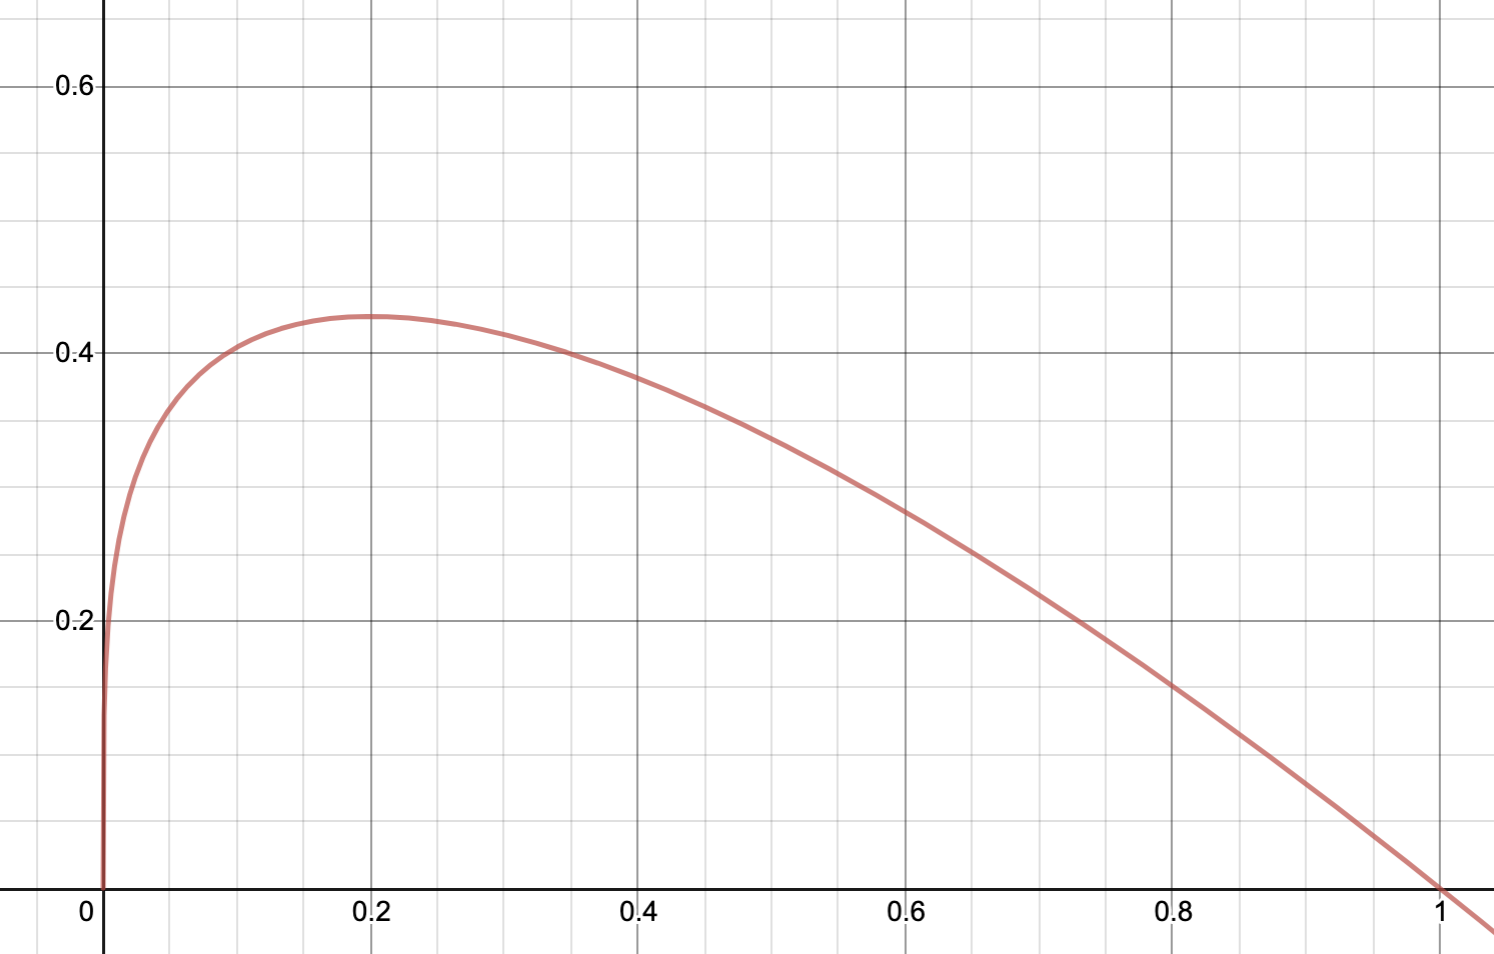
\includegraphics[width=6cm]{ps3fig1}
   \caption{Graph of $g$ in terms of $\gamma$. $\alpha$ set to 0.8}
 \end{centering}
\end{figure}
\problempart{(7)}
Plugging in the consumption law of motion, we get the government tries to maximize
\[ \int_0^\infty \frac{\left(k(0) e^{g(\gamma)t} ((1-\gamma)\alpha A(\gamma) - g(\gamma)) \right)^{1-\theta} - 1}{1-\theta} e^{-\rho t} \]
Removing terms with no $\gamma$ dependence, we need to maximize
\[ \frac{\left(k(0)((1-\gamma)\alpha A(\gamma) - g(\gamma))\right)^{1-\theta}}{(1-\theta)((1-\theta)g(\gamma) - \rho)} \]
Taking the first derivative wrt $\gamma$, we have
\[ \frac{k(0)\left(k(0)((1-\gamma)\alpha A(\gamma) - g(\gamma))\right)^{-\theta} \left((1-\theta)g(\gamma) - \rho)\left(\alpha(1-\gamma)A'(\gamma)-\alpha A(\gamma) - g'(\gamma)\right) - \left((1-\gamma)\alpha A(\gamma) - g(\gamma)\right)  g'(\gamma)\right)}{((1-\theta)g(\gamma) - \rho)^2} \]
Take $\gamma = 1-\alpha$. We know from the previous part that $g'(\gamma) = 0$, so
\[ \frac{k(0) \left((1-\theta)g(\gamma) - \rho)\left(\alpha (1-\alpha) A(\gamma)/\gamma -\alpha A(\gamma)\right) \right)}{((1-\theta)g(\gamma) - \rho)^2\left(k(0)((1-\gamma)\alpha A(\gamma) - g(\gamma))\right)^{\theta}} \]

\[ =\frac{k(0) \left((1-\theta)g(\gamma) - \rho)\left(\alpha A(\gamma) -\alpha A(\gamma)\right) \right)}{((1-\theta)g(\gamma) - \rho)^2\left(k(0)((1-\gamma)\alpha A(\gamma) - g(\gamma))\right)^{\theta}} \]

\[ =\frac{k(0) \left((1-\theta)g(\gamma) - \rho)0\right)}{((1-\theta)g(\gamma) - \rho)^2\left(k(0)((1-\gamma)\alpha A(\gamma) - g(\gamma))\right)^{\theta}} \]
\[ = 0 \]
Hence the growth maximizing choice of $\gamma$ is also welfare optimal. Intuitively, this makes sense; growth and welfare are both trying to maximize $(1-\gamma)A$, and so optimizing one also optimizes the other.
\problempart{(8)}
The government should tax labor where possible, and finance the remainder with taxes on capital. Since the labor supply is inelastic and consumers do not have utility for leisure in this model, taxing labor as much as possible minimizes impact of the tax.
\problempart{(9)}

Assuming firms treat the government spending as exogenous, we have
\[ G_t = \gamma Y_t = \gamma k_t^\alpha G_t^{\xi(1-\alpha)} L_t^{1-\alpha} \]
\[ G_t ^{1 - \xi(1-\alpha)} = \gamma k_t^\alpha L_t^{1-\alpha} \]
\[ G_t = (\gamma L_t^{1-\alpha})^{1/(1 - \xi(1-\alpha))} k_t^{\alpha/(1 - \xi(1-\alpha))} \]
Rewriting output, we get
\[ Y_t =k_t^\alpha G_t^{1-\alpha} L_t^{1-\alpha} \]
\[=  k_t^\alpha L_t^{1-\alpha} (\gamma L_t^{1-\alpha})^{\xi(1-\alpha)/(1 - \xi(1-\alpha))} k_t^{\xi(1-\alpha)\alpha/(1 - \xi(1-\alpha))} \]
\[ = (\gamma L_t)^{\xi(1-\alpha)/(1 - \xi(1-\alpha))} k_t^{\alpha /(1 - \xi(1-\alpha))} \]
which is the standard neoclassical form, as long as $\xi < 1$, converging to steady state, no growth.
\pagebreak
\problem{3}

\problempart{(1)}
No. $\dot{h}/h$ will be decreasing in $h$, and hence the growth rate drops, so long-run growth cannot be sustained.
\problempart{(2)}
The household problem is
\[ \max \int e^{-\rho t} \frac{c(t)^{1-\theta} - 1}{1-\theta} \]
subject to
\[ \dot{h}(t) = \delta h(t)(1-u(t)) \]
\[ \dot{k}(t) = k(t)^\beta (u(t)h(t))^{1-\beta}\bar{h}(t)^\gamma - c(t) \]
The current value Hamiltonian is
\[ H = \frac{c(t)^{1-\theta} - 1}{1-\theta} + \lambda(t)\delta h(t)(1-u(t)) + \mu(t) (k(t)^\beta (u(t)h(t))^{1-\beta}\bar{h}(t)^\gamma - c(t)) \]
The FOCs:
\[ \frac{\partial H}{\partial c} = c^{-\theta} - \mu = 0 \]
\[ \frac{\partial H}{\partial h} = \lambda \delta (1-u) + \mu (1-\beta) k^\beta (uh)^{-\beta}u\bar{h}^\gamma = \rho \lambda - \dot{\lambda} \]
\[ \frac{\partial H}{\partial u} = - \lambda \delta h + \mu (1-\beta)k^\beta (uh)^{-\beta}h \bar{h}^\gamma = 0  \]
\[ \frac{\partial H}{\partial k} = \mu \beta k^{\beta - 1}(u h )^{1-\beta}\bar{h}^\gamma = \rho \mu - \dot{\mu} \]
\problempart{(3)}
From the first FOC, we get
\[ \frac{\dot{c}}{c}= -\frac{1}{\theta} \frac{\dot{\mu}}{\mu} \]
From the fourth, we have
\[ k^{\beta - 1}(u h )^{1-\beta}\bar{h}^\gamma - \rho = - \frac{\dot{\mu}}{\mu} \]
Combining, we get
\[ \frac{\dot{c}}{c}= \frac{1}{\theta} \left( \beta k^{\beta - 1}(u h )^{1-\beta}\bar{h}^\gamma - \rho  \right) \]
\[ = \frac{1}{\theta} \left( \beta k^{\beta - 1}u^{1-\beta}h^{1-\beta+\gamma} - \rho  \right)  \]

\problempart{(4)}
\[ g_h = \frac{\dot{h}}{h} = \delta (1-u) \]
Since in equilibrium
\[ y = k^\beta (uh)^{1-\beta}\bar{h}^\gamma = k^\beta u^{1-\beta}h^{1-\beta + \gamma}\]
\[ \dot{y} = \beta k^{\beta - 1}\cdot{k} u^{1-\beta}h^{1-\beta + \gamma} + (1-\beta + \gamma )k^\beta u^{1-\beta}h^{-\beta + \gamma} \]

\[ g_y = \beta g_k  + (1-\beta + \gamma )g_h \]
Taking $g_k = g_c = g_y$, we get
\[ g_k = g_c = \frac{1-\beta + \gamma}{1-\beta}\delta (1-u) \]
\problempart{(5)}
We need to find the steady state $u$. From the 3rd FOC:
\[ \lambda \delta h = \mu (1-\beta)k^\beta u^{-\beta}h^{1 - \beta + \gamma}  \]
\[ g_\lambda + g_h = g_\mu + \beta g_k + (1-\beta+\gamma) g_h  \]
From FOC 2:
\[  \rho - \delta (1-u) - (\mu/\lambda) (1-\beta) k^\beta (uh)^{-\beta}u\bar{h}^\gamma = g_\lambda \]
Since from FOC 3
\[ \frac{\delta h}{(1-\beta)k^\beta u^{-\beta}h^{1 - \beta + \gamma}} = \mu/\lambda   \]
Plugging in we get
\[  \rho - \delta (1-u) - \delta u = g_\lambda \]
\[  \rho - \delta  = g_\lambda \]
We already know
\[ g_c = -\frac{1}{\theta} g_\mu \]
So aall together we get
\[ g_\lambda + g_h = g_\mu + \beta g_k + (1-\beta+\gamma) g_h  \]
\[ \rho - \delta   = - \theta g_c + \beta g_k + (\gamma - \beta) g_h  \]
Using
\[ g_c = g_k = \frac{1-\beta + \gamma}{1-\beta} g_h \]
we get
\[ \rho - \delta   =  \left( (\beta - \theta)\frac{1-\beta + \gamma}{1-\beta} + \gamma - \beta \right)  g_h  \]
\[ g_h  =  \frac{(\rho - \delta )(1-\beta)}{ \gamma - \theta(1-\beta + \gamma) }    \]
\[ u^* = 1 - \frac{(\rho - \delta )(1-\beta)}{ \delta (\gamma - \theta(1-\beta + \gamma) )}  \]

\[ g_c = g_k  =  \frac{(\rho - \delta )(1-\beta+\gamma)}{ \gamma - \theta(1-\beta + \gamma) }    \]

\problempart{(6)}
Since $\bar{h}$ is no longer exogenous, the second FOC changes to

\[ \frac{\partial H}{\partial h} = \lambda \delta (1-u) + \mu (1-\beta + \gamma) k^\beta u^{1-\beta}h^{-\beta+\gamma} = \rho \lambda - \dot{\lambda} \]
\[ \delta (1-u) + (\mu/\lambda) (1-\beta + \gamma) k^\beta u^{1-\beta}h^{-\beta+\gamma} = \rho  - g_\lambda \]
\[ \rho - \delta  -
\frac{ \gamma}{1-\beta} \delta u   = g_\lambda \]
\[ \rho - \delta -
\frac{ \gamma}{1-\beta} \delta  = \left((\beta- \theta) \frac{1-\beta + \gamma}{1-\beta} + \left(\gamma - \beta + \frac{\gamma}{1-\beta}\right) \right) g_h  \]
\[ (\rho - \delta)(1-\beta) -
\gamma \delta  = \left((\beta- \theta) (1-\beta + \gamma) + (\gamma - \beta)(1-\beta)  - \gamma  \right) g_h  \]

\[ \frac{\gamma \delta - (\rho - \delta)(1-\beta)
}{\theta (1-\beta + \gamma)}  =  g_h  \]

\[ \frac{\gamma \delta - (\rho - \delta)(1-\beta)
}{\theta (1-\beta)}  =  g_c = g_k  \]

These are different from the results in part 5, and the social planner would accumulate human capital faster. One way to induce efficiency in the previous result would be to provide some subsidy for $1-u$ to encourage education.
\pagebreak
\problem{4}

\problempart{(1)}
The problem is
\[ \max \log c_1(t) + \beta \log c_2(t) \]
subject to
\[ c_1(t) + s(t) \le w(t) \]
\[ c_2(t) \le s(t)R(t+1) \]
\problempart{(2)}
The firm problem FOCs:
\[ w(t) = (1-\alpha) A(t)K(t)^\alpha L(t)^{-\alpha} \]
\[ R(t) = \alpha A(t)K(t)^{\alpha-1} L(t)^{1-\alpha} \]
\problempart{(3)}
\begin{itemize}
  \item Households solve the household optimization problem.
  \item Firms solve the firm profit maximization problem
  \item Markets clear: $K(t+1) = s(t)L(t)$
\end{itemize}
A steady state equilibrium is a competitive equilibrium where $y, k$
grow at constant rates
\problempart{(4)}
From the firm problem above, we get
\[ \frac{1}{c_1} = \lambda \]
\[ \frac{\beta}{c_2} = \mu \]
\[ \lambda = \mu R(t+1) \]
\[ \frac{1}{c_1} = R(t+1)\frac{\beta}{c_2} \]
\[ \beta  c_1 = s \]
\[ s(t) = \frac{\beta w(t)}{1+\beta} \]
\[ c_1(t) = \frac{w(t)}{1+\beta}  \]
\[ c_2(t) =  \frac{\beta R(t+1)w(t)}{1+\beta} \]
So the law of motion of capital is
\[ k(t+1) = \frac{\beta w(t)}{(1+\beta)(1+n)} = \frac{\beta (1-\alpha) A(t)k(t)^\alpha}{(1+\beta)(1+n)} \]
\problempart{(5)}
Taking $\hat{k}$ as suggested, we have from the law of motion:
\[ k(t+1) = \frac{\beta (1-\alpha) A(t)k(t)^\alpha}{(1+\beta)(1+n)} \]
\[ k(t)(1+g)^{1/(1-\alpha)} = \frac{\beta (1-\alpha) A(t)k(t)^\alpha}{(1+\beta)(1+n)} \]
\[ 1 = \frac{\beta (1-\alpha) A(t)k(t)^{\alpha-1}}{(1+\beta)(1+n)(1+g)^{1/(1-\alpha)}} \]
\[ 1  = \frac{\beta (1-\alpha) (\hat{k}^*)^{\alpha-1}}{(1+\beta)(1+n)(1+g)^{1/(1-\alpha)}} \]

\[ (\hat{k}^*)^{1-\alpha}  = \frac{\beta (1-\alpha) }{(1+\beta)(1+n)(1+g)^{1/(1-\alpha)}} \]
\[\hat{k}^*   = \left(\frac{\beta (1-\alpha) }{(1+\beta)(1+n)(1+g)^{1/(1-\alpha)}} \right)^{1/(1-\alpha)} \]
By the problem hint, capital grows at $(1+g)^{1/(1-\alpha)}$. Since capital is linearly related to $c_1, s, w$, it follows that all of these also grow at the same rate. Also, since $R$ is determined entirely by $\hat{k}$, since this is constant, $R$ is also constant. Hence $c_2$ also grows at the same rate as capital.
\problempart{(6)}
The law of motion for $\hat{k}$ takes the form
\[ \hat{k}(t+1) = C\hat{k}(t)^\alpha \]
where $C$ is some constant in terms of $\beta, n, \alpha, g$. Then we note that for $\hat{k} > \hat{k}^*$, since $\alpha < 1$, $\hat{k}(t)^\alpha$ is concave, so $ \hat{k} > C\hat{k}^\alpha > \hat{k}^*$. So when $\hat{k}$ is above $\hat{k}^*$, it will decrease to the steady state. The similar argument holds when $\hat{k} < \hat{k}^*$, so the equilibrium we found in the previous part is globally stable.
\problempart{(7)}
By examining the expression for $\hat{k}^*$, we note this shifts down, and since $R$ depends inversely on $\hat{k}^*$, $R$ increases. Additionally, since the growth rate of $k$ increases, $k$ shifts up. Since at steady state equilibrium, $w, s, c_1, c_2$ are linearly dependent on $k$, all of these also all shift up.
\pagebreak
\problem{5}

\problempart{(1)}
The equilibrium wage is
\[ w(t) = \left( (aK(t))^{\frac{\epsilon-1}{\epsilon}} + 1 \right)^{\frac{1}{\epsilon - 1}} \]
The equilibrium return to capital is
\[ R(t) = \frac{a}{(aK(t))^{1/\epsilon}}\left( (aK(t))^{\frac{\epsilon-1}{\epsilon}} + 1 \right)^{\frac{1}{\epsilon - 1}} \]
\problempart{(2)}
\[ \frac{w}{Y} = \left( (aK(t))^{\frac{\epsilon-1}{\epsilon}} + 1 \right)^{-1} \]
as $K(t)$ increases, since $\epsilon > 1$, the parenthesized expression increases and hence the labor share decreases.
\problempart{(3)}
In a competitive equilibrium:
\begin{itemize}
  \item Household solves consumer problem:
  \[ \max \log c_1(t) + \beta \log c_2(t) \]
  subject to
  \[ c_1(t) + s(t) \le w(t) \]
  \[ c_2(t) \le s(t)R(t+1) \]
  \item Firms maximize profits, so wages and capital return rates are set as in part 1.
  \item Markets clear: $K(t+1) = s(t)$
\end{itemize}
Since the utility is a variant of Cobb-Douglas, we get
\[ s(t) = \frac{\beta w(t)}{1+\beta} \]
So capital evloves as
\[ K(t+1) = \frac{\beta}{1+\beta} \left( (aK(t))^{\frac{\epsilon-1}{\epsilon}} + 1 \right)^{\frac{1}{\epsilon - 1}} \]
The steady state level of capital $K^*$ then solves

\[ K^* = \frac{\beta}{1+\beta} \left( (aK^*)^{\frac{\epsilon-1}{\epsilon}} + 1 \right)^{\frac{1}{\epsilon - 1}} \]
\problempart{(4)}
The modified law of motion is

\[ K(t+1) = \frac{\beta}{1+\beta}\sigma \left( (aK(t))^{\frac{\epsilon-1}{\epsilon}} + 1 \right)^{\frac{\epsilon}{\epsilon - 1}} \]
\[ K(t+1)^{\frac{\epsilon-1}{\epsilon}} = \left(\frac{\beta}{1+\beta}\sigma\right)^{\frac{\epsilon-1}{\epsilon}} \left( a^{\frac{\epsilon-1}{\epsilon}}K(t)^{\frac{\epsilon-1}{\epsilon}} + 1 \right) \]
\[ K(t+1)^{\frac{\epsilon-1}{\epsilon}} =  \left(\frac{\beta}{1+\beta}\sigma\right)^{\frac{\epsilon-1}{\epsilon}} a^{\frac{\epsilon-1}{\epsilon}}K(t)^{\frac{\epsilon-1}{\epsilon}} + \left(\frac{\beta}{1+\beta}\sigma\right)^{\frac{\epsilon-1}{\epsilon}}  \]
\[ K(t+1)^{\frac{\epsilon-1}{\epsilon}} =  \left(\frac{\beta}{1+\beta}\sigma a\right)^{\frac{\epsilon-1}{\epsilon}} K(t)^{\frac{\epsilon-1}{\epsilon}} + \left(\frac{\beta}{1+\beta}\sigma\right)^{\frac{\epsilon-1}{\epsilon}}  \]
Since $\sigma a \beta / (1+\beta) > 1$, the sequence of $K(t)^{\frac{\epsilon-1}{\epsilon}}$ grows at a constant rate. There isn't a steady state, but a steady growth equilibrium. See the figure for diagram.
\begin{figure}
\begin{centering}
\begin{tikzpicture}
\draw[thick,->] (0,0) -- (8,0) node[anchor=north west] {$k$};
\draw[thick,->] (0,0) -- (0,8) node[anchor=south east] {$k'$};
\draw (0,0) -- (8,8) node[anchor=south west] {$k=k'$};
\draw[blue] (0,0) -- (6,8) node[anchor=south east] {Constant wage share of output};
\draw[red] (0,0) .. controls (1,3) .. (8,5) node[anchor=south west] {Competitive wage};
\end{tikzpicture}
\caption{Question 5, Part 4}
\end{centering}
\end{figure}
\problempart{(5)}
The economy in (4) has long-run balanced growth, so it is richer in the long run than the economy in (3), which eventually stops growing at steady-state.
\end{document}
	% line of code telling latex that your document is ending. If you leave this out, you'll get an error
